%\documentstyle[epsf,twocolumn]{jarticle}       %LaTeX2.09仕様
%\documentclass[twocolumn]{jarticle}     %pLaTeX2e仕様
\documentclass{jarticle}     %pLaTeX2e仕様

%一枚組だったら[twocolumn]関係のとこ消す

\setlength{\topmargin}{-45pt}
%\setlength{\oddsidemargin}{0cm} 
\setlength{\oddsidemargin}{-7.5mm}
%\setlength{\evensidemargin}{0cm} 
\setlength{\textheight}{24.1cm}
%setlength{\textheight}{25cm} 
\setlength{\textwidth}{17.4cm}
%\setlength{\textwidth}{172mm} 
\setlength{\columnsep}{11mm}

\kanjiskip=.07zw plus.5pt minus.5pt

\usepackage{graphicx}
\usepackage[dvipdfmx]{color}
\usepackage{subcaption}
\usepackage{enumerate}
\usepackage{comment}
\usepackage{url}
\usepackage{multirow}
\usepackage{diagbox}


\begin{document}
  \onecolumn
  \noindent
  \hspace{1em}

  \today
  \hfill
  \ \  B3 西村昭賢 

  \vspace{2mm}
  \hrule
  \begin{center}
  {\Large \bf 情報工学実験2 10/18課題}
  \end{center}
  \hrule
  \vspace{3mm}


\section*{タイトル}
不完全情報ゲームにおける強化学習を用いた戦略の構築とその分析\cite{1}

\section*{著者}
阿部慎太郎,竹川高志

\section*{何に関する研究か}
プレイヤーに与えられる情報が部分的である不完全情報ゲームでは,駆け引きが生じるため必勝手は存在しない.また,不完全情報ゲームの中でもプロ選手が生まれていることから無数にある戦略の中でも総合的な優劣があると考えられる.\par
この研究では,このような不完全情報ゲームにおいて平均的に勝つことができる戦略の構築を目指している.
実験の際に使用する不完全情報ゲームとしては,5枚のカードverの「ハゲタカのえじき」を採用している.図1に「ハゲタカのえじき」のゲームの流れを示す.\par

\begin{figure}[ht]
  \centering
  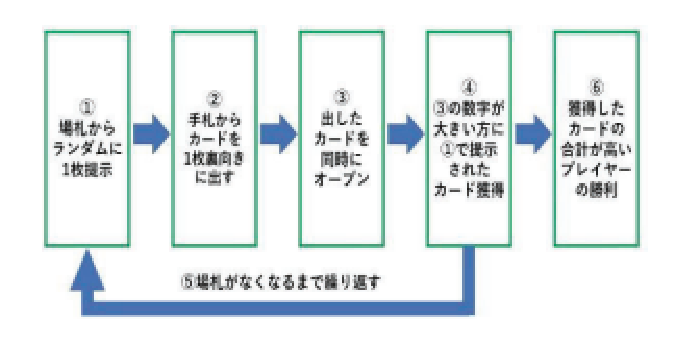
\includegraphics[width=120mm]{assets/Figure1.eps}
  \caption{「ハゲタカのえじき」のゲームの流れ}
  \label{fig:GameFlow of HAGETAKA}
\end{figure}



\section*{実験内容}
この章がないと筆者の主張や興味深い点がが伝わりにくいと考えたため追加した.\par
強化学習を用いて特定の対戦相手との対戦からcounter戦略を作成する.不完全情報ゲームには平均的に勝つことのできる強い戦略が存在するという仮定に基づき,counter戦略の対戦を繰り返すことでより強い戦略の構築を目指す.\par
実験の際には,手札からランダムにカードを出すrandom戦略,バフだと同じカードを数字から出す固定戦略,DQNを用いて相手との対戦から学習を行いカウンターとなる行動を選択するcounter戦略,複数の戦略の中から対戦ごとに強い戦略を多く選択するように戦略を切り替える切り替え戦略の4つの戦略を設定した.
また,本研究ではcounter戦略 vs random戦略の対戦,counter戦略 vs 固定戦略の対戦を行っている.\par

\subsection*{counter戦略 vs random戦略}
counter戦略 vs random戦略の対戦では,ランダム戦略との対戦を繰り返して学習したcounte\_random戦略を構築した.

\subsection*{counter戦略 vs 固定戦略}
counter戦略 vs 固定戦略の対戦では,まず,counter戦略 vs 固定戦略の対戦から学習し,counter\_1戦略を作成した.同様にcounter\_1戦略の対戦から学習したcounter\_2戦略を作成し,固定,counter\_1,counter\_2の3つの戦略でグループを構築し,グループの総当りから勝率の割合を計算し,切り替え戦略\_1を作成する.そして,counter戦略と切り替え戦略\_1の対戦から学習したcounter\_mix1戦略をグループに追加する.この流れを図2のように繰り返してcounter\_mix7戦略まで作成した.

\begin{figure}[ht]
  \centering
  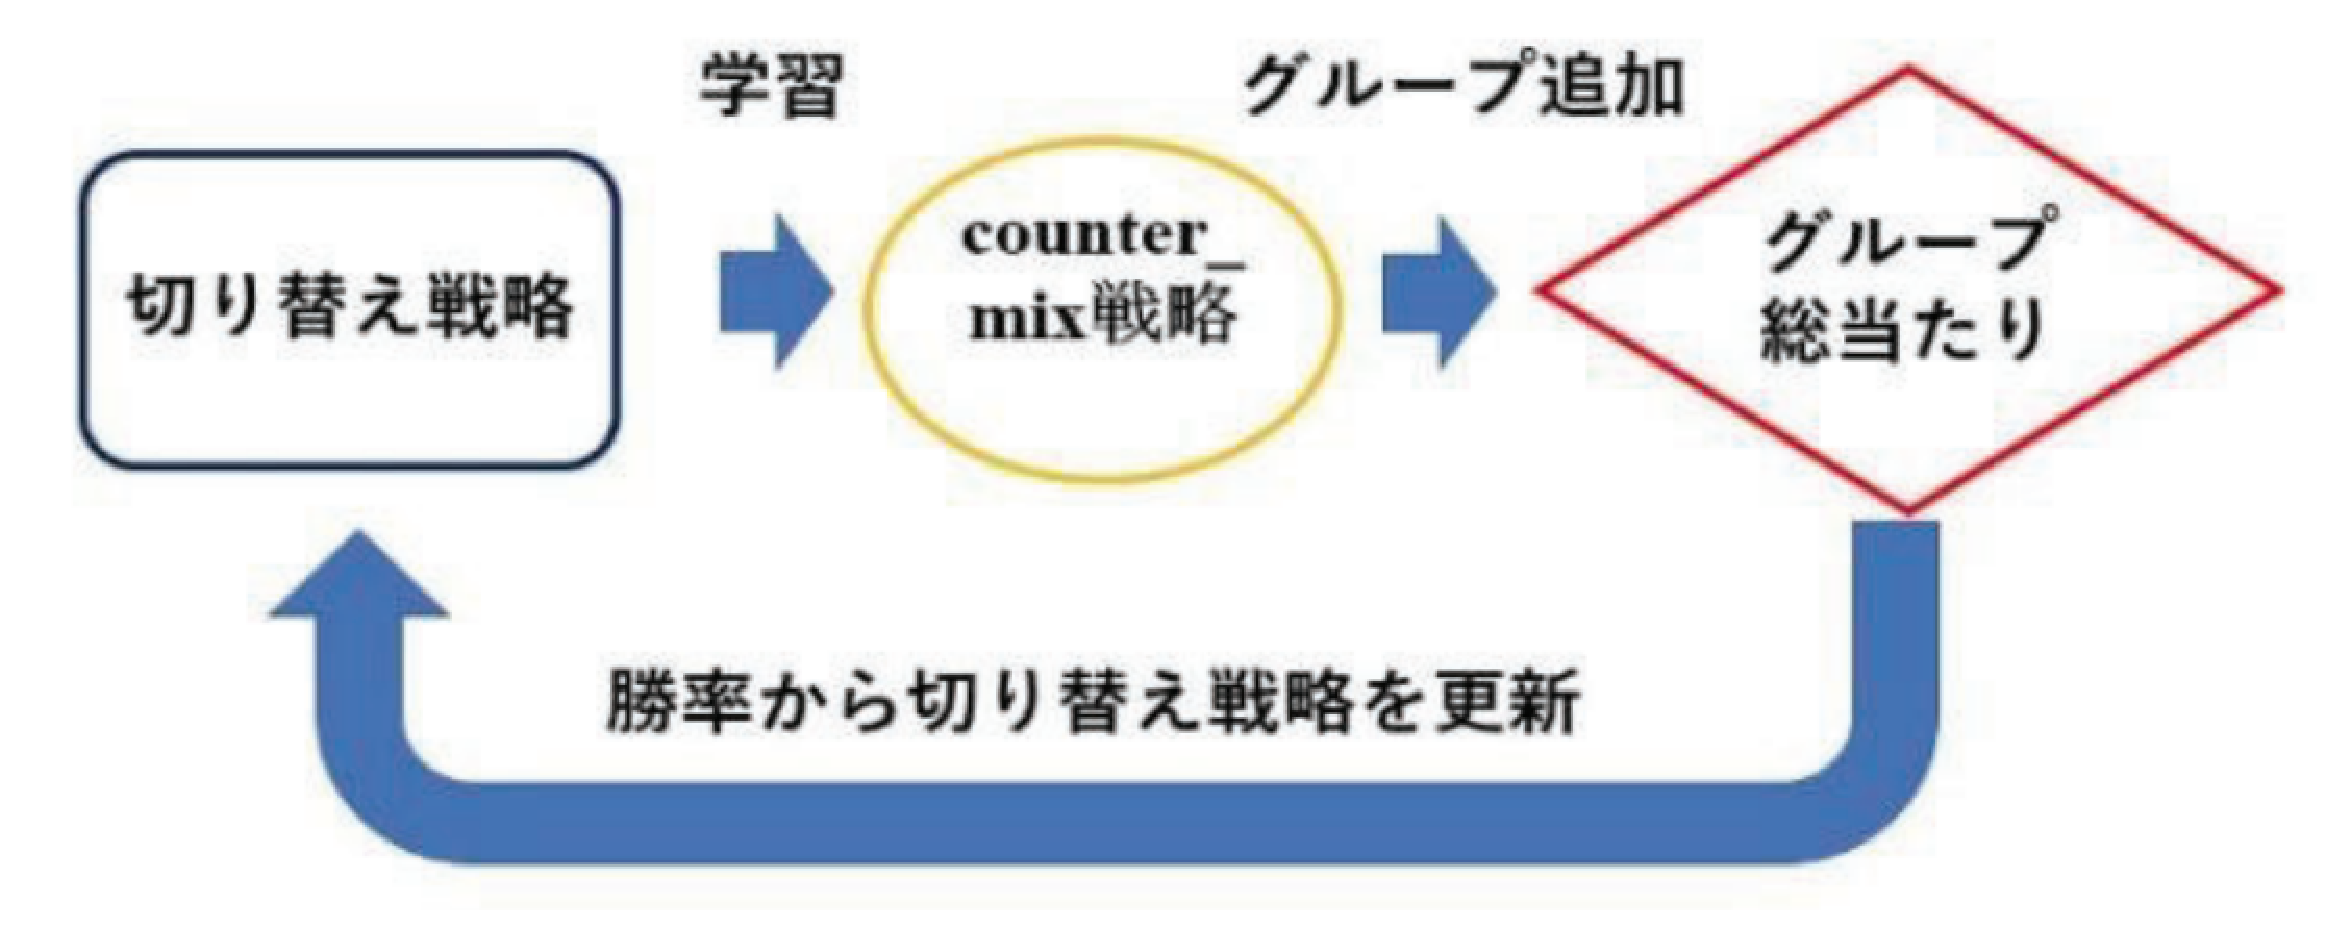
\includegraphics[width=120mm]{assets/Figure2.eps}
  \caption{固定戦略を基にしたグループの作成方法}
  \label{fig:How to nake grouping}
\end{figure}


\section*{著者が主張している点}


\subsection*{counter戦略 vs random戦略}
counter\_random戦略はrandom戦略に対して約88\%場札と同じ数字のカードを手札から出す傾向があることが判明した.すなわちrandom戦略には固定戦略が有効であることが判明した.
\subsection*{counter戦略 vs 固定戦略}
counter戦略に関しては1つ前の戦略にはどの戦略も90\%以上の勝率になった.また,最も新しい世代の戦略であるcounter\_mix7戦略はグループ内のすべての戦略に対して勝率が60\%以上となった.\par
また,このcounter\_mix7戦略の行動における各ゲーム情報の重要度を決定木分析で行った.各ゲーム情報は自分の手札,相手の手札,残りの場札,得点差であり,結果としてcounter\_mix7戦略は得点差と残りの場札に関する情報の重要度が高く,各プレイヤーの手札に関する情報の重要度は低くなった.
\subsection*{結論と今後の課題}
\par
このように,対戦相手に合わせた強化学習により,対戦相手に平均的に勝つことのできるゲームAIの構築が可能だと言える.
\par
本研究では予め対戦相手の戦略を設定していたが,ゲームの途中で戦略を変更する,あえて弱い行動をして駆け引きに持ち込むなど複雑な戦略相手に勝利するためには情報の集約や対戦相手の特徴の把握などの学習の際の工夫が必要である.人間との対戦から効率よく学習を行い,平均的に勝つことのできる戦略を探求していく.

\section*{興味深い点}

\subsection*{counter\_mix7戦略の戦略決定の情報}
不完全情報ゲーム,特に本実験の「ハゲタカのえじき」では,相手の手札というプレイヤーに与えられない情報が存在する.決定木分析により得られたcounter\_mix7戦略の戦略決定において,他プレイヤーの手札という本来得られない情報の重要度は低く,得点差と残りの場札といった盤面から取得可能な情報の重要度は高くなっていた.この情報の重み付けが学習の際に最適化された結果であるかどうかは本論文では明かされていないが,counter\_mix7戦略が盤面の情報から戦略を組み立てて一定の成果を上げていることが面白かった.

\subsection*{切り替え戦略を用いたcounter\_mix戦略の作成}
counter\_2戦略を作った後に図2のように戦略を同一グループに入れ,切り替え戦略を作成し学習を行っていた.単純にcounter\_2戦略を作成後にcounter\_2戦略と固定戦略を学習させてcounter\_3戦略を作成する方法では恐らく過学習の問題が起こるため本研究はこのような方法にしたと考えたが,興味深い実験方法だなと感じた.

\section*{この次に読むべき資料}



\subsection*{自分が理解できてなかったキーワード}

\begin{quote}
  \begin{itemize}
   \item AlphaGo \par
   \url{https://www.nature.com/articles/nature16961}
   \item DeepBlue\par
   \url{https://cir.nii.ac.jp/crid/1050845762805286016}
   \item 決定木分析\par
   \url{https://qiita.com/3000manJPY/items/ef7495960f472ec14377}
  \end{itemize}
 \end{quote}

\subsection*{より複雑なゲームの学習}

\begin{quote}
  \begin{itemize}
   \item AlphaSter(stercraft2を解くAI) \par
   \url{https://www.deepmind.com/blog/alphastar-mastering-the-real-time-strategy-game-starcraft-ii}
  \end{itemize}
 \end{quote}

\subsection*{不完全情報ゲームの深層強化学習応用例}

\begin{quote}
  \begin{itemize}
   \item 逆転オセロニアへの応用\par
   \url{https://www.ipsj.or.jp/dp/contents/publication/38/S1002-S05.html}
  \end{itemize}
 \end{quote}





%index.bibはtexファイルと同階層に置く
%ちゃんと\citeしないと表示されない(1敗)
\bibliography{index.bib}
\bibliographystyle{junsrt}

\end{document}